
\section*{Supplemental material}


\subsection{InfoGAN based Model}
The intuitions gained from the experiments performed for the non-parametric density estimation led to the Gated Residual Block on the Generator of a GAN. InfoGAN \cite{chen2016infogan} presented a perfect setting to apply the Gated Residual Block in the case of the generator. The first set of experiments were on MNIST and Fashion-MNIST with sets of 10 discrete variables (since there were 10 classes in both of the datasets) and 2 continuous variables whose information was tried to be maximized using the Q network. As can be seen in \figref{fig:infogan_unconditional} the network was able to generate realistic images from the different classes and produce meaningful interpolations by varying the continuous variables as shown in the figure. The exact experimental setting was that the hypernetwork responsible for the predictions of the $alpha^i$s which we term as the gate selection network gets the salient variables and has no information about the random noise sampled for the main network(consisting of gated residual blocks), based on the salient variables received the gate selection network predicts the  $alpha^i$s for all the blocks of the network. The main network is oblivious of the conditioning received in the salient variables and has to generate images coherent with the conditioning since the Q-Network tries to reconstruct back the conditioning received in the form of salient variables. 

\begin{figure}[t]%[ht!]
    \centering
    \addSubFigHalf{Picture35}{MNIST}{fig:infogan_mnist} 
    \addSubFigHalf{Picture34}{Fashion-MNIST}{fig:infogan_fashion_mnist} 
    \caption{Gated Residual Block-InfoGAN on MNIST and Fashion MNIST \ow{do we have the standard infogan comparison here?}}
    \label{fig:infogan_unconditional}
    \vspace{-3mm}
\end{figure}

\subsection{Unconditional Generations}
\begin{figure}[t]
    \centering
    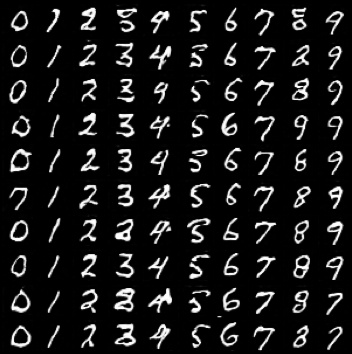
\includegraphics[width=0.5\linewidth]{Picture5}
    \caption{Results on the Gated Residual Block on MNIST dataset}\label{fig:grb_mnist}
    \vspace{-4mm}
\end{figure}

A well known problem in image conditional GAN settings is the tendency to produce realistic outputs but not being able to produce meaningful variations in the generated output. It was especially prevalent in the original pix2pix setting \cite{isola2016image2image} and further research enabled variations such as \cite{ghosh2017multi} and \cite{zhu2017toward}. Although as shown in \cite{ghosh2017multi} the naive infoGAN setting couldn't produce meaningful variations in the pix2pix setting, settling rather for very minute variations. Our Gated Residual Blocks could mitigate some of the problems and did produce variations in the challenging task of edges-to-bag generation as has been demonstrated in \figref{fig:infogan_bags}. By varying the continuous variable smooth interpolations could be obtained between colors and textures which was earlier not possible with the infogan based pix2pix setting. Although the variations along the discrete axis was quite minimal and we are still investigating the cause for the same. The experimental setting in this scenario was that the salient variables were only given to the gate selection network and had to predict the $alpha^i$s for the main network which consisted of gated residual blocks and was oblivious of the conditioning provided in the form of salient variables. The Discriminator network was the standard image conditional discriminator network while the Q network in this scenario was modified to take the generated image as well as the edge map to behave as a image conditional Q Network which tries to reconstruct back the salient variables given to the gate selection network. 

\newcommand{\addSubFigEighth}[3]{\begin{subfigure}[t]{.18\linewidth}
   \includegraphics[width=\linewidth]{#1}
   \caption{#2}\label{#3}\end{subfigure}
}
\newcommand{\addSubFigEighthCaptionless}[3]{\begin{subfigure}[t]{.18\linewidth}
   \includegraphics[width=\linewidth]{#1}
   \label{#2}\end{subfigure}
}

The next set of experiments were performed to judge the robustness of the Gate Selection Blocks and the Gated Residual Blocks in the case the labels were available. That meant using the gate selection network and the gated residual blocks on the discriminator. The implications were even more interesting, the gate selection network would have to distribute the blocks between the classes to get the class specific gradients back for training the class conditioned generator. In the unconditional setting for the generator, the main block only receives random noise and the gate selection block receives the class condition and predicts the $aplha^i$s for the gated residual blocks. The discriminator on the other hand is composed of a main network consisting of gated residual blocks which is oblivious to the class conditioning and a gate selection network which predicts the $aplha^i$s for the main network of the discriminator. The main network predicts how real/fake an image is based on the alpha weightings of its gated residual blocks. The network is able to disentangle the class conditioning although none of the main networks of the generator/ discriminator are aware of the class conditioning, the class information only being input to the gate selection network which has to modulate the weights of the respective networks' gated residual blocks. The generated samples on the MNIST dataset are shown in \figref{fig:grb_mnist} and the alpha gatings for the different classes and the different blocks in \figref{fig:mnist_act}. The values for the gates clearly show switching off of certain blocks in the case it is not needed for a particular class even though a sparsity constraint was not applied in the training objective.


\begin{figure}%[ht!]
    \centering
    \addSubFigHalf{Picture6}{Activations of the gated residual blocks in the generator}{fig:gen_act} 
    \addSubFigHalf{Picture7}{Activations of the gated residual blocks in the discriminator}{fig:dis_act} 
    \caption{Activation of the various blocks in the Generator and Discriminator}
    \label{fig:mnist_act}
    \vspace{-3mm}
\end{figure}






\begin{figure*}[t]%[ht!]
    \centering
    \addSubFigEighthCaptionless{Picture8}{Sketch}{fig:bag_sketch} 
    \addSubFigEighthCaptionless{Picture9}{Varition 1}{fig:bag_1} 
    \addSubFigEighthCaptionless{Picture10}{Varition 2}{fig:bag_2}
    \addSubFigEighthCaptionless{Picture11}{Varition 3}{fig:bag_3}
    \addSubFigEighthCaptionless{Picture12}{Varition 4}{fig:bag_4}
    \caption{The variations produced in the sketch to realistic bag task in the infogan with Gated Residual Block setting for the generator }
    \label{fig:infogan_bags}
    \vspace{-3mm}
\end{figure*}




\subsection{1-D network architecture}

\begin{table}[ht]
\caption{Resblock} % title of Table
\centering % used for centering table
\begin{tabular}{c} % centered columns (4 columns)
\hline\hline %inserts double horizontal lines
F(x)\\%heading
\hline % inserts single horizontal line
Linear(nneurons,nneurons)\\ % inserting body of the table
ReLU() \\
Linear(nneurons,nneurons) \\
\hline %inserts single line
\end{tabular}
\label{table:resblock} % is used to refer this table in the text
\end{table}


\begin{table}[ht]
\caption{\textbf{Generator for 1D setting}} % title of Table
\centering % used for centering table
\begin{tabular}{c c} % centered columns (4 columns)
\hline\hline %inserts double horizontal lines
layer & num layers\\%heading
\hline % inserts single horizontal line
Linear(10,4) & 1\\ % inserting body of the table
ResBlock(4) & 16 \\
Linear(4,1) & 1 \\
\hline %inserts single line
\end{tabular}
\label{table:1d_G} % is used to refer this table in the text
\end{table}

\begin{table}[ht]
\caption{\textbf{Discriminator for 1D setting}} % title of Table
\centering % used for centering table
\begin{tabular}{c c} % centered columns (4 columns)
\hline\hline %inserts double horizontal lines
layer & num layers\\%heading
\hline % inserts single horizontal line
Linear(1,4) & 1\\ % inserting body of the table
ResBlock(4) & 16 \\
Linear(4,1) & 1 \\
Sigmoid & 1 \\
\hline %inserts single line
\end{tabular}
\label{table:1d_D} % is used to refer this table in the text
\end{table}



\subsection{Outline$\rightarrow$Image Network Architecture}

\begin{table}[ht]
\caption{\textbf{ConvResblock}} % title of Table
\centering % used for centering table
\begin{tabular}{c} % centered columns (4 columns)
\hline\hline %inserts double horizontal lines
F(x)\\%heading
\hline
Conv2d(nfilters,kernel=3,stride=1,padding=1) \\
InstanceNorm2d(nfilters)\\ % inserting body of the table
ReLU() \\
Conv2d(nfilters,kernel=3,stride=1,padding=1) \\
InstanceNorm2d(nfilters)\\ % inserting body of the table
ReLU() \\
\hline %inserts single line
\end{tabular}
\label{table:convresblock} % is used to refer this table in the text
\end{table}


\begin{table}[ht]
\caption{\textbf{UpConvResblock}} % title of Table
\centering % used for centering table
\begin{tabular}{c} % centered columns (4 columns)
\hline\hline %inserts double horizontal lines
F(x)\\%heading
\hline
Upsample (Nearest Neighbor) \\
ReflectionPad2d(1) \\
Conv2d(nfilters,kernel=3,stride=1,padding=0) \\
InstanceNorm2d(nfilters)\\ % inserting body of the table
ReLU() \\
Conv2d(nfilters,kernel=3,stride=1,padding=1) \\
InstanceNorm2d(nfilters)\\ % inserting body of the table
ReLU() \\
\hline %inserts single line
Shortcut\\
\hline 
Upsample (Nearest Neighbor) \\
ReflectionPad2d(1)\\
Conv2d(nfilters,kernel=3,stride=1,padding=0) \\
\hline
\end{tabular}
\label{table:upconvresblock} % is used to refer this table in the text
\end{table}

\begin{table}[ht]
\caption{\textbf{DownConvResblock}} % title of Table
\centering % used for centering table
\begin{tabular}{c} % centered columns (4 columns)
\hline\hline %inserts double horizontal lines
F(x)\\%heading
\hline
Avgpool 2d \\
ReflectionPad2d(1) \\
Conv2d(nfilters,kernel=3,stride=1,padding=0) \\
InstanceNorm2d(nfilters)\\ % inserting body of the table
ReLU() \\
Conv2d(nfilters,kernel=3,stride=1,padding=1) \\
InstanceNorm2d(nfilters)\\ % inserting body of the table
ReLU() \\
\hline %inserts single line
Shortcut\\
\hline 
Avgpool 2d \\
ReflectionPad2d(1)\\
Conv2d(nfilters,kernel=3,stride=1,padding=0) \\
\hline
\end{tabular}
\label{table:downconvresblock} % is used to refer this table in the text
\end{table}


\begin{table}[ht]
\caption{\textbf{Gated Resnet G:Scribble Dataset}}
\centering % used for centering table
\begin{tabular}{c} % centered columns (4 columns)
\hline
Conv2d(3,64,kernel=3,stride=1,padding=1) \\
InstanceNorm2d(64)\\ % inserting body of the table
ReLU() \\
\hline %inserts single line
3xGatedConvResBlock(64) \\
3xDownGatedConvResBlock(64) \\
12xGatedConvResBlock(64) \\
3xUpGatedConvResBlock(64) \\
3xGatedConvResBlock(64) \\
\hline
Conv2d(64,3,kernel=3,stride=1,padding=1) \\
Tanh() \\
\hline
\end{tabular}
\label{table:resnet_g_scribble} % is used to refer this table in the text
\end{table}

\begin{table}[ht]
\caption{\textbf{Gated Resnet D:Scribble Dataset}} % title of Table
\centering % used for centering table
\begin{tabular}{c} % centered columns (4 columns)
\hline
Conv2d(6,64,kernel=3,stride=1,padding=1) \\
\hline %inserts single line
3xGatedConvResBlock(64) \\
4xDownGatedConvResBlock(64) \\
17xGatedConvResBlock(64) \\
\hline
Conv2d(64,1,kernel=3,stride=1,padding=1) \\
Sigmoid() \\
\hline
\end{tabular}
\label{table:resnet_d_scribble} % is used to refer this table in the text
\end{table}



% \begin{figure*}%[ht!]
%     \centering
%     \addSubFigTenth{acgan_baseline_all/basketball_11_real_A}{}{fig:basketball_scribble} 
%     \addSubFigTenth{acgan_baseline_all/chicken_2_real_A}{}{fig:chicken_scribble} 
%     \addSubFigTenth{acgan_baseline_all/cookie_13_real_A}{}{fig:cookie_scribble}
%     \addSubFigTenth{acgan_baseline_all/cupcake_27_real_A}{}{fig:cupcake_scribble}
%     \addSubFigTenth{acgan_baseline_all/moon_15_real_A}{}{fig:moon_scribble}
%     \addSubFigTenth{acgan_baseline_all/basketball_11_fake_B}{}{fig:basketball_img} 
%     \addSubFigTenth{acgan_baseline_all/chicken_2_fake_B}{}{fig:chicken_img} 
%     \addSubFigTenth{acgan_baseline_all/cookie_13_fake_B}{}{fig:cookie_img}
%     \addSubFigTenth{acgan_baseline_all/cupcake_27_fake_B}{}{fig:cupcake_img}
%     \addSubFigTenth{acgan_baseline_all/moon_15_fake_B}{}{fig:moon_img}
%     \addSubFigTenth{acgan_baseline_all/orange_17_real_A}{}{fig:orange_scribble} 
%     \addSubFigTenth{acgan_baseline_all/pineapple_2_real_A}{}{fig:pineapple_scribble} 
%     \addSubFigTenth{acgan_baseline_all/soccer_18_real_A}{}{fig:soccer_scribble}
%     \addSubFigTenth{acgan_baseline_all/strawberry_1_real_A}{}{fig:strawberry_scribble}
%     \addSubFigTenth{acgan_baseline_all/watermelon_17_real_A}{}{fig:watermelon_scribble}
%     \addSubFigTenth{acgan_baseline_all/orange_17_fake_B}{}{fig:orange_img} 
%     \addSubFigTenth{acgan_baseline_all/pineapple_2_fake_B}{}{fig:pineapple_img} 
%     \addSubFigTenth{acgan_baseline_all/soccer_18_fake_B}{}{fig:soccer_img}
%     \addSubFigTenth{acgan_baseline_all/strawberry_1_fake_B}{}{fig:strawberry_img}
%     \addSubFigTenth{acgan_baseline_all/watermelon_17_fake_B}{}{fig:watermelon_img}
%     \caption{ACGAN baseline with Input Provided to all layers of Generator}
%     \label{fig:scribble_pix2pix}
%     \vspace{-3mm}
% \end{figure*}


% \begin{figure*}%[ht!]
%     \centering
%     \addSubFigTenth{channel_gated/basketball_11_real_A}{}{fig:basketball_scribble} 
%     \addSubFigTenth{channel_gated/chicken_2_real_A}{}{fig:chicken_scribble} 
%     \addSubFigTenth{channel_gated/cookie_13_real_A}{}{fig:cookie_scribble}
%     \addSubFigTenth{channel_gated/cupcake_27_real_A}{}{fig:cupcake_scribble}
%     \addSubFigTenth{channel_gated/moon_15_real_A}{}{fig:moon_scribble}
%     \addSubFigTenth{channel_gated/basketball_11_fake_B}{}{fig:basketball_img} 
%     \addSubFigTenth{channel_gated/chicken_2_fake_B}{}{fig:chicken_img} 
%     \addSubFigTenth{channel_gated/cookie_13_fake_B}{}{fig:cookie_img}
%     \addSubFigTenth{channel_gated/cupcake_27_fake_B}{}{fig:cupcake_img}
%     \addSubFigTenth{channel_gated/moon_15_fake_B}{}{fig:moon_img}
%     \addSubFigTenth{channel_gated/orange_17_real_A}{}{fig:orange_scribble} 
%     \addSubFigTenth{channel_gated/pineapple_2_real_A}{}{fig:pineapple_scribble} 
%     \addSubFigTenth{channel_gated/soccer_18_real_A}{}{fig:soccer_scribble}
%     \addSubFigTenth{channel_gated/strawberry_1_real_A}{}{fig:strawberry_scribble}
%     \addSubFigTenth{channel_gated/watermelon_17_real_A}{}{fig:watermelon_scribble}
%     \addSubFigTenth{channel_gated/orange_17_fake_B}{}{fig:orange_img} 
%     \addSubFigTenth{channel_gated/pineapple_2_fake_B}{}{fig:pineapple_img} 
%     \addSubFigTenth{channel_gated/soccer_18_fake_B}{}{fig:soccer_img}
%     \addSubFigTenth{channel_gated/strawberry_1_fake_B}{}{fig:strawberry_img}
%     \addSubFigTenth{channel_gated/watermelon_17_fake_B}{}{fig:watermelon_img}
%     \caption{Gated (Channel/Alpha) Results}
%     \label{fig:scribble_pix2pix}
%     \vspace{-3mm}
% \end{figure*}


% \begin{figure*}%[ht!]
%     \centering
%     \addSubFigSixthLabel{channel_gated/basketball_11_real_A}{Basketball}{fig:basketball_input} 
%     \addSubFigSixth{channel_gated/basketball_11_fake_B}{fig:basketball_ours} 
%     \addSubFigSixth{block_gated/basketball_11_fake_B}{fig:basketball_block}
%     \addSubFigSixth{channel_gated_affine/basketball_11_fake_B}{fig:basketball_channel_affine}
%     \addSubFigSixth{block_gated_affine/basketball_11_fake_B}{fig:basketball_block_affine}
%     \addSubFigSixth{adain/basketball_11_fake_B}{fig:basketball_adain}
    
%     \addSubFigSixthLabel{channel_gated/soccer_18_real_A}{Soccer ball}{fig:soccer_input}
%     \addSubFigSixth{channel_gated/soccer_18_fake_B}{fig:soccer_ours} 
%     \addSubFigSixth{block_gated/soccer_18_fake_B}{fig:soccer_block}
%     \addSubFigSixth{channel_gated_affine/soccer_18_fake_B}{fig:soccer_channel_affine}
%     \addSubFigSixth{block_gated_affine/soccer_18_fake_B}{fig:soccer_block_affine}
%     \addSubFigSixth{adain/soccer_18_fake_B}{fig:soccer_adain}
    
%     \addSubFigSixthLabel{channel_gated/moon_15_real_A}{Moon}{fig:moon_input}
%     \addSubFigSixth{channel_gated/moon_15_fake_B}{fig:moon_ours} 
%     \addSubFigSixth{block_gated/moon_15_fake_B}{fig:moon_block}
%     \addSubFigSixth{channel_gated_affine/moon_15_fake_B}{fig:moon_channel_affine}
%     \addSubFigSixth{block_gated_affine/moon_15_fake_B}{fig:moon_block_affine}
%     \addSubFigSixth{adain/moon_15_fake_B}{fig:moon_adain}
    
    
%     \addSubFigSixthLabel{channel_gated/cookie_13_real_A}{Cookie}{fig:cookie_input}
%     \addSubFigSixth{channel_gated/cookie_13_fake_B}{fig:cookie_ours} 
%     \addSubFigSixth{block_gated/cookie_13_fake_B}{fig:cookie_block}
%     \addSubFigSixth{channel_gated_affine/cookie_13_fake_B}{fig:cookie_channel_affine}
%     \addSubFigSixth{block_gated_affine/cookie_13_fake_B}{fig:cookie_block_affine}
%     \addSubFigSixth{adain/cookie_13_fake_B}{fig:cookie_adain}
    
    
%     \addSubFigSixthLabel{channel_gated/orange_17_real_A}{Orange}{fig:orange_input}
%     \addSubFigSixth{channel_gated/orange_17_fake_B}{fig:orange_ours} 
%     \addSubFigSixth{block_gated/orange_17_fake_B}{fig:orange_block}
%     \addSubFigSixth{channel_gated_affine/orange_17_fake_B}{fig:orange_channel_affine}
%     \addSubFigSixth{block_gated_affine/orange_17_fake_B}{fig:orange_block_affine}
%     \addSubFigSixth{adain/orange_17_fake_B}{fig:orange_adain}
    
%     \addSubFigSixthLabel{channel_gated/watermelon_17_real_A}{Watermelon}{fig:watermelon_input}
%     \addSubFigSixth{channel_gated/watermelon_17_fake_B}{fig:watermelon_ours} 
%     \addSubFigSixth{block_gated/watermelon_17_fake_B}{fig:watermelon_block}
%     \addSubFigSixth{channel_gated_affine/watermelon_17_fake_B}{fig:watermelon_channel_affine}
%     \addSubFigSixth{block_gated_affine/watermelon_17_fake_B}{fig:watermelon_block_affine}
%     \addSubFigSixth{adain/watermelon_17_fake_B}{fig:watermelon_adain}
    
%     \addSubFigSixthLabel{channel_gated/cupcake_27_real_A}{Cupcake}{fig:cupcake_input}
%     \addSubFigSixth{channel_gated/cupcake_27_fake_B}{fig:cupcake_ours} 
%     \addSubFigSixth{block_gated/cupcake_27_fake_B}{fig:cupcake_block}
%     \addSubFigSixth{channel_gated_affine/cupcake_27_fake_B}{fig:cupcake_channel_affine}
%     \addSubFigSixth{block_gated_affine/cupcake_27_fake_B}{fig:cupcake_block_affine}
%     \addSubFigSixth{adain/cupcake_27_fake_B}{fig:cupcake_adain}
    
    
%     \addSubFigSixthLabel{channel_gated/strawberry_1_real_A}{Strawberry}{fig:strawberry_input}
%     \addSubFigSixth{channel_gated/strawberry_1_fake_B}{fig:strawberry_ours} 
%     \addSubFigSixth{block_gated/strawberry_1_fake_B}{fig:strawberry_block}
%     \addSubFigSixth{channel_gated_affine/strawberry_1_fake_B}{fig:strawberry_channel_affine}
%     \addSubFigSixth{block_gated_affine/strawberry_1_fake_B}{fig:strawberry_block_affine}
%     \addSubFigSixth{adain/strawberry_1_fake_B}{fig:strawberry_adain}
    
%     \addSubFigSixthLabel{channel_gated/chicken_2_real_A}{Fried Chicken}{fig:chicken_input}
%     \addSubFigSixth{channel_gated/chicken_2_fake_B}{fig:chicken_ours} 
%     \addSubFigSixth{block_gated/chicken_2_fake_B}{fig:chicken_block}
%     \addSubFigSixth{channel_gated_affine/chicken_2_fake_B}{fig:chicken_channel_affine}
%     \addSubFigSixth{block_gated_affine/chicken_2_fake_B}{fig:chicken_block_affine}
%     \addSubFigSixth{adain/chicken_2_fake_B}{fig:chicken_adain}
    
%     \caption{Various Gating Mechanisms}
%     \label{fig:multi-task_cityscapes}
%     \vspace{-3mm}
% \end{figure*}